% !TeX root = thesis.tex

\chapter{Evaluation}
\label{ch:evaluation}
This chapter will evaluate the performance of the previously discussed \velocity{} framework. In the first section, the two projects that will be used in the subsequent experiments will be presented. The next section will formally restate the research questions that have been posed in the introduction and extend these. Afterwards, the procedure of how the data was obtained will be elaborated. The final section will provide answers to the research questions as well as present the results of applying \tcp{} to the test subjects.

% !TeX root = ../thesis.tex

\section{Test subjects}

\subsection{Dodona}
Dodona\footnote{\url{https://dodona.ugent.be/}} is an open-source online learning environment created by Ghent University, which allows students from secondary schools and universities in Belgium and South-Korea to submit solutions to programming exercises and receive instant, automated feedback. The application is built using the Ruby-on-Rails web framework. To automate the testing process of the application, Dodona employs \githubactions{} (\cref{sssec:github-actions}) which executes the more than $\SI{450}{}$ test cases in the test suite and performs static code analysis. The application is tested using the default \texttt{MiniTest} testing framework and \texttt{SimpleCov}\footnote{\url{https://github.com/colszowka/simplecov}} is used to record the coverage of the test suite, which is currently approximately $\SI{89}{\percent}$.

\subsection{Stratego}
The second test subject is an application which was created for the Software Engineering Lab 2 course at Ghent University in 2018. The application was created for a Belgian gas transmission system operator and consists of two main components: a web frontend and a backend. This thesis will test the backend in particular since it is written in Java using the Spring framework. Furthermore, the application uses Gradle and JUnit to execute the $\SIrange{300}{400}{}$ test cases in the test suite, allowing the Java agent (\cref{ssec:velocity-frontend}) to be applied directly.
% !TeX root = ../thesis.tex

\section{Research questions}
We will answer the following research questions in the subsequent sections:

\paragraph*{RQ1: What is the probability that a test run will contain at least one failed test case?}
The first research question will provide useful insights into whether a typical test run tends to fail or not. The expectancy is that the probability of failure will be rather low, indicating that it is not strictly necessary to execute every test case and therefore making a case for \tsm{}.

\paragraph*{RQ2: What is the average duration of a test run?}
Measuring how long it takes to execute a typical test run is required to estimate the benefit of applying any form of test suite optimisation. We will only consider successful test runs, to reduce bias introduced by prematurely aborting the execution.

\paragraph*{RQ3: Suppose that a test run has failed, what is the probability that the next run will fail as well?}
The ROCKET algorithm (\cref{ssec:alg-rocket}) relies on the assumption that if a test case has failed in a given test run, it is likely to fail in the subsequent run as well. This research question will investigate the likelihood of this hypothesis.

\paragraph*{RQ4: How can \tcp{} be applied to Dodona and what is the resulting performance benefit?}
This research question will investigate the possibility to apply the \velocity{} framework to the Dodona project and analyse how quickly the available predictors can discover a failing test case.

\paragraph*{RQ5: Can the Java agent be applied to Stratego?}
Since the testing framework used by Stratego should be supported natively by the Java agent, this research question will verify its compatibility. Furthermore, we will analyse the prediction performance, albeit with a small number of relevant test runs.
% !TeX root = ../thesis.tex

\section{Data collection}\label{sec:eval-data}

% !TeX root = ../../thesis.tex

\subsection{\travisci{} build data}
In order to answer the first three research questions, build data for several projects hosted on \travisci{} (\autoref{sssec:travisci}) was used. This data was obtained from two sources.\\

\noindent The first source is a database of $\SI{35793144}{}$ jobs, provided by Durieux et al \cite{travisanalysis}. Due to the magnitude of this dataset ($\SI{61.11}{\gibi\byte}$), a big data framework is required to parse the log files. In order to collect the required data to provide an answer to the first and third research question, two simple \texttt{MapReduce} pipelines have been executed using the Apache Spark\footnote{\url{https://spark.apache.org/}} framework..\\

\begin{figure}[htbp!]
	\centering
	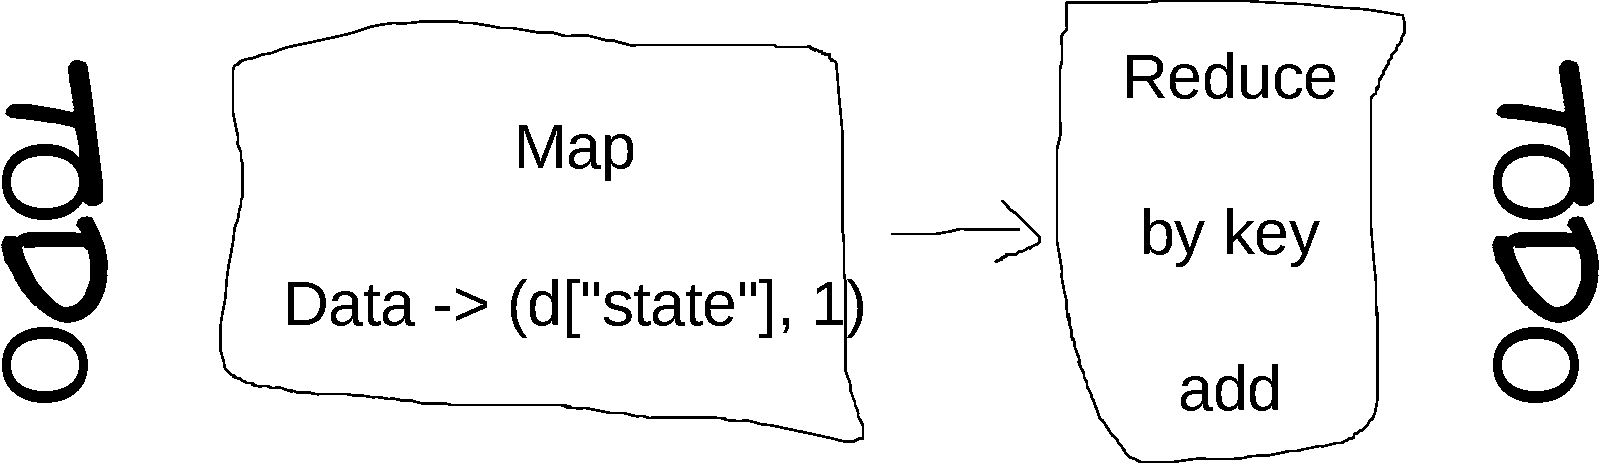
\includegraphics[width=0.8\textwidth]{assets/images/eval-rq1-mapreduce.pdf}
	\caption{MapReduce pipeline to find the failed runs}
	\label{fig:eval-mapreduce-1}
\end{figure}

\begin{figure}[htbp!]
	\centering
	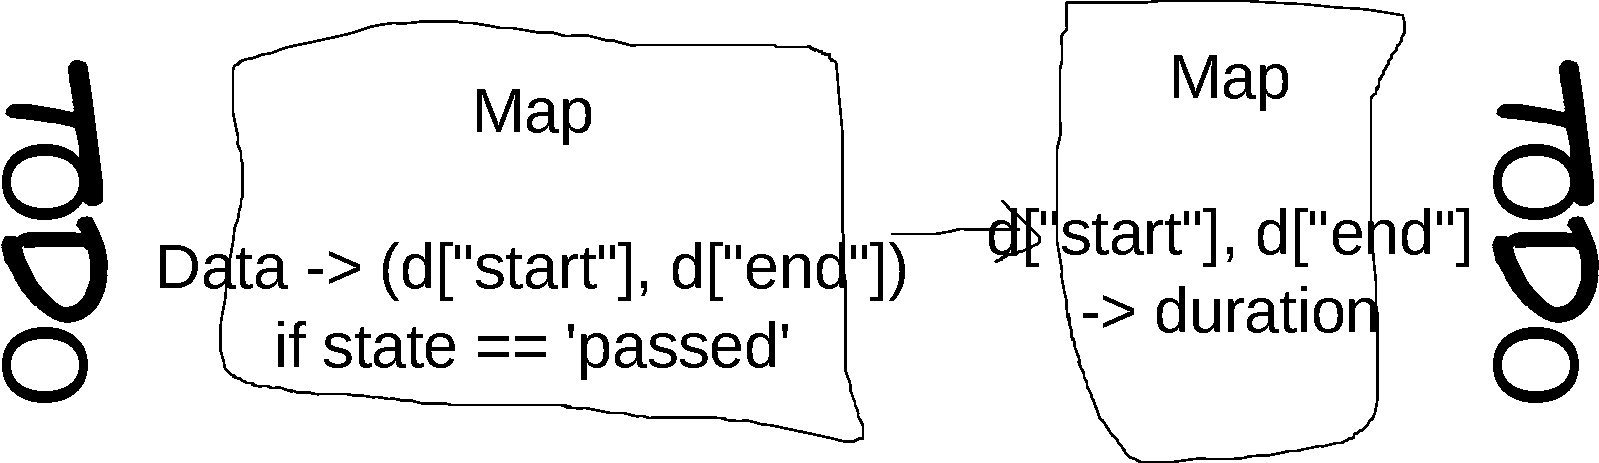
\includegraphics[width=0.8\textwidth]{assets/images/eval-rq3-mapreduce.pdf}
	\caption{MapReduce pipeline to find the average duration of a successful test run}
	\label{fig:eval-mapreduce-3}
\end{figure}

\noindent In addition to the first source, another $\SI{3702595}{}$ jobs have been analysed from the \emph{TravisTorrent} project. This project \cite{msr17challenge} scrapes the API of \travisci{} and combines this with data obtained from the \github{} API to augment the dataset with extra information. One of these additional values is the identifier of the previous executed build of every project. This identifier is required to answer the second research question. Furthermore, the amount of failed test cases in every run is included, which can be used to distinguish whether the test run has actually failed or the project could not be compiled and thus allowing a more fine-grained answer to the first research question as well. After analysis of this dataset, the execution time was not accurate compared to the actual timings on the \travisci{} build page, so this dataset was not used in the third research question. For analysis, the creators of TravisTorrent have provided a Google BigQuery\footnote{\url{https://bigquery.cloud.google.com/}} interface to allow querying the dataset, which is required given its magnitude. The following queries have been executed to obtain the required data:

\lstinputlisting[caption=TravisTorrent query: Find the amount of failed runs, label=lst:travistorrent-sql1, language=sql]{assets/listings/travistorrent-failed-runs.sql}
\lstinputlisting[caption=TravisTorrent query: Find the probability of consecutive failures,label=lst:travistorrent-sql2, language=sql]{assets/listings/travistorrent-consecutive-failures.sql}

% !TeX root = ../../thesis.tex

\subsection{Dodona data}
As mentioned before, Dodona utilises the MiniTest testing framework in conjunction with SimpleCov to calculate the coverage. MiniTest will by default only emit the name of every failed test case, without any further information. Furthermore, SimpleCov is only capable of calculating the coverage for the entire test suite and does not allow to retrieve the coverage on a per-test basis. To answer the fourth research question and apply the \velocity{} predictors to Dodona, a Python script has been created to reconstruct every failed test run. This script first queries the API of \githubactions{} to find which test runs have failed. In this thesis, $\SI{62}{}$ failed runs have been used. For every failed commit, the script retrieves the parent commit and calculates the coverage on a per-test basis. This thesis will assume that the coverage of the parent commit resembles the coverage of the failed commit. The coverage is calculated by applying the following two transformations to the parent commits and subsequently rescheduling these in \githubactions{}:

\begin{itemize}
	\item \textbf{Cobertura formatter:} The current SimpleCov reports can only be generated as HTML reports, preventing convenient analysis. This problem is resolved by using the Cobertura formatter instead, which generates XML reports. The structure of these reports is already supported by the Controller.
	
	\item \textbf{Parallel execution:} To reduce the execution time, the test cases are concurrently executed by four processes. The code coverage is recorded per process and afterwards merged. However, SimpleCov is not entirely thread-safe. This is not a problem if the total coverage is required, but it does prevent the accurate generation of per-test coverage. As a result, parallel execution has been disabled.
	
\end{itemize}
% !TeX root = ../thesis.tex

\section{Results}

\subsection{RQ1: Probability of failure}\label{ssec:results-rq1}
\autoref{fig:rq1-failure-probability} contains two pie charts that illustrate the amount of failed and successful test runs. The left chart contains the results of the dataset provided by Durieux et al \cite{travisanalysis}. This dataset contains $\SI{4558279}{}$ failed test runs versus $\SI{24323724}{}$ successful runs, which corresponds to a failure probability of $\SI{18.74}{\percent}$. The other pie chart visualises data from the TravisTorrent project. According to this dataset, the run has failed prior to starting the test suite in $\SI{42.89}{\percent}$ of the executions. For the remaining part of the runs, $\SI{225766}{}$ out of $\SI{2114920}{}$ executions contained at least one failed test case, corresponding to a failure percentage of $\SI{10.67}{\percent}$.

\begin{figure}[htbp!]
	\centering
	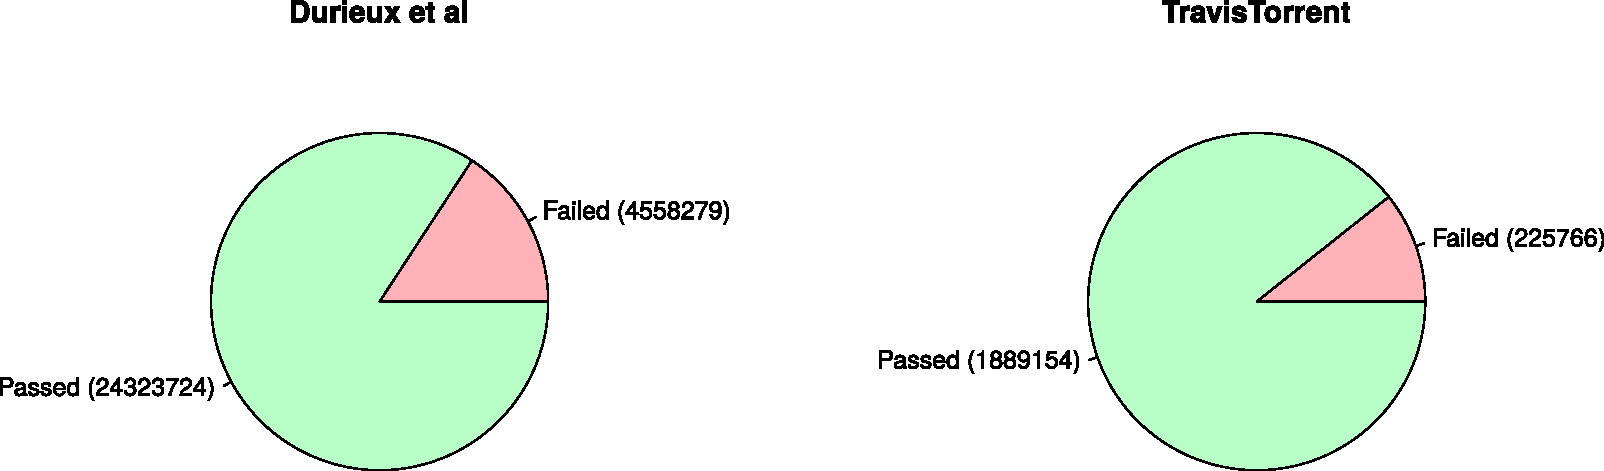
\includegraphics[width=\textwidth]{assets/charts/rq1-failure-probability.pdf}
	\caption{Probability of test run failure}
	\label{fig:rq1-failure-probability}
\end{figure}

\subsection{RQ2: Probability of consecutive failure}
In order to find consecutive failures, only the TravisTorrent project can be used as every entry in this dataset contains the identifier of the previous build which is required to link consecutive builds. The dataset contains $\SI{211040}{}$ test runs of which the test suite of the preceding test run was both executed and contained at least one failed test case. As illustrated in \autoref{fig:rq2-consecutive-failure}, $\SI{109224}{}$ of these test runs failed as well, versus $\SI{101816}{}$ test runs ($\SI{51.76}{\percent}$) that did succeed.

\begin{figure}[htbp!]
	\centering
	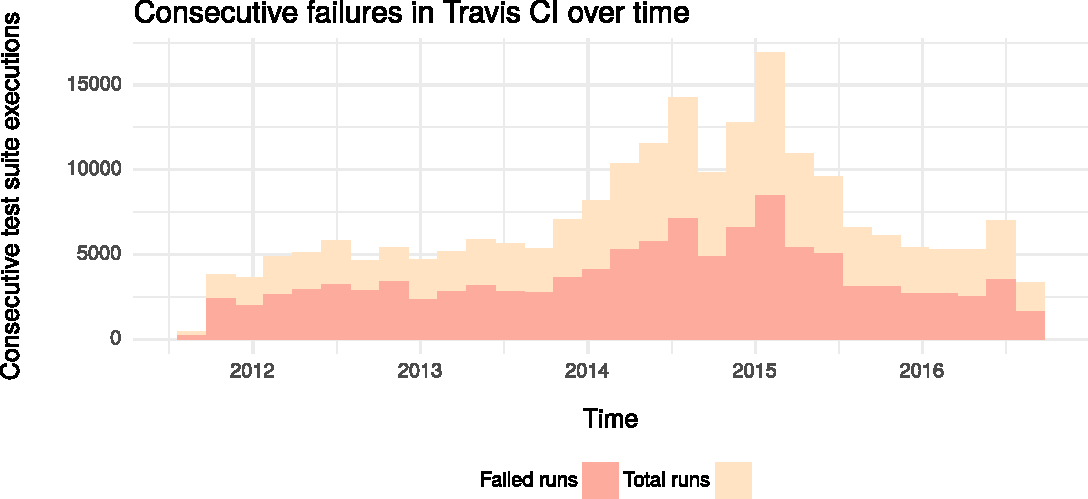
\includegraphics[width=\textwidth]{assets/charts/rq2-consecutive-failure.pdf}
	\caption{Consecutive test run failures on \travisci{}}
	\label{fig:rq2-consecutive-failure}
\end{figure}

\subsection{RQ3: Average test run duration}
The \travisci{} dataset provided by Durieux et al \cite{travisanalysis} has been filtered to exclude test runs with an execution time of less than $\SI{10}{\second}$, as this generally implies that the test suite did not actually execute due to an initialisation failure. \autoref{tbl:rq3-characteristics} contains the characteristics of the remaining analysed test runs. This table suggests that \travisci{} is primarily used for small projects, yet the maximal value is a strong outlier. \autoref{fig:rq3-durations} confirms the existence of $\SI{71378}{}$ test runs with an execution time of more than one hour. Further investigation has pointed out that these are mostly projects which are using mutation testing (\autoref{sssec:mutation-testing}), such as \texttt{plexus/yaks}\footnote{A Ruby library for hypermedia (\url{https://github.com/plexus/yaks}).}.

\begin{table}[h]
	\centering
	\begin{tabularx}{\textwidth}{|C|C|C|C|C|}
		\hline
		\textbf{\# runs} & \textbf{Minimum} & \textbf{Mean} & \textbf{Median} & \textbf{Maximum}\\
		\hline
		$\SI{24320504}{}$ & $\SI{10}{\second}$ & $\SI{385}{\second}$ & $\SI{178}{\second}$ & $\SI{26}{\hour} \SI{11}{\minute} \SI{26}{\second}$\\
		\hline
	\end{tabularx}
	\caption{Characteristics of the test run durations in \cite{travisanalysis}.}
	\label{tbl:rq3-characteristics}
\end{table}

\begin{figure}[htbp!]
	\centering
	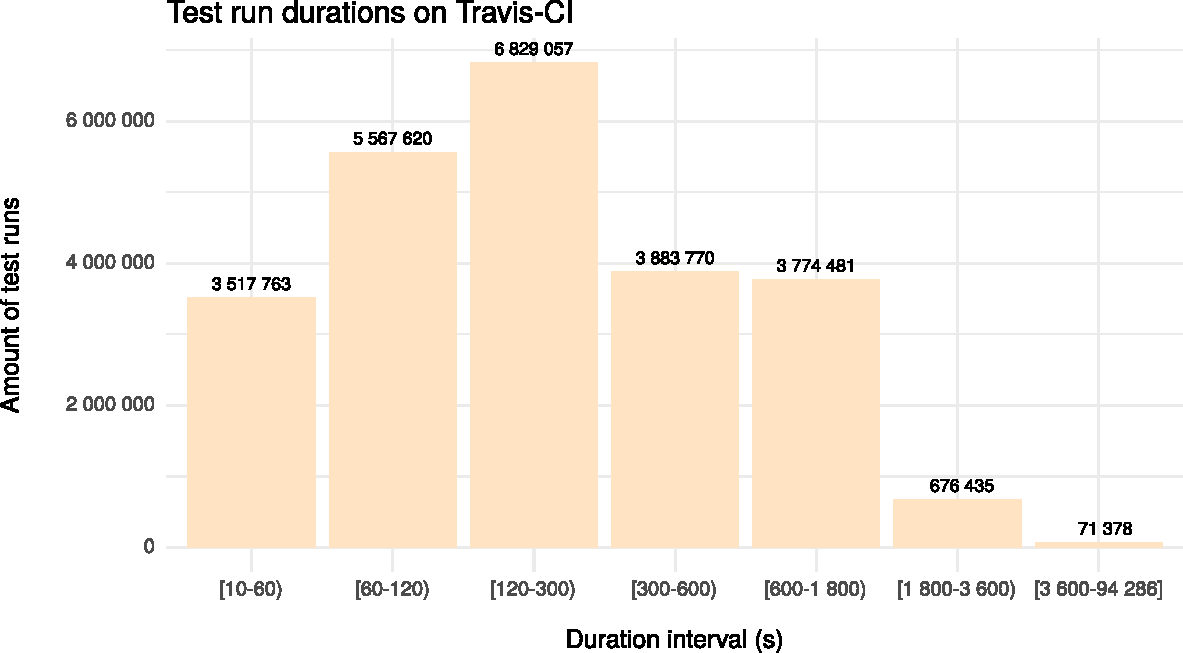
\includegraphics[width=\textwidth]{assets/charts/rq3-test-run-durations.pdf}
	\caption{Test run durations on \travisci{}}
	\label{fig:rq3-durations}
\end{figure}


\subsection{RQ4: Applying \tcp{} to Dodona}
Given the $\SI{62}{}$ collected test runs, another $\SI{9}{}$ runs have been omitted because these have been identified as a bug in the configuration of the test suite, preventing any test to be executed at all. This is something which cannot be detected by a prioritisation framework, since this requires more contextual information about the project.\\

\noindent \autoref{fig:rq4-performance} compares the performance of respectively the Alpha algorithm, the Greedy algorithm, the HGS algorithm and the ROCKET algorithm to the original, non-prioritised execution. The Alpha and HGS algorithm provide the most accurate predictions, with the latter algorithm being the least consistent. The Greedy algorithm on the other hand succeeds in predicting some executions very accurately, while failing to predict other runs anywhere near, which is the expected behaviour of a greedy heuristic. Finally, the ROCKET algorithm is not suitable for this project.\\

\begin{figure}[htbp!]
\centering
\subfloat[Alpha algorithm]{%
	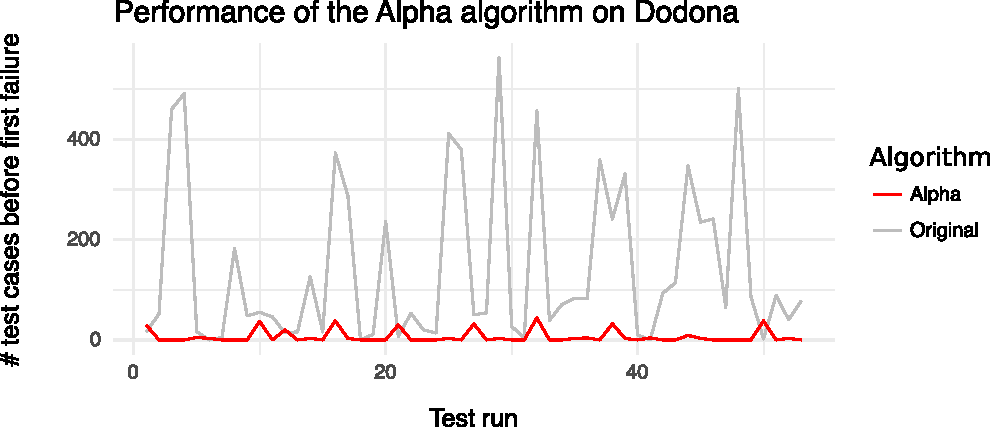
\includegraphics[width=\textwidth]{assets/charts/rq4-dodona-alpha.pdf}
}
\end{figure}
\begin{figure}
\ContinuedFloat
\subfloat[Greedy algorithm]{%
	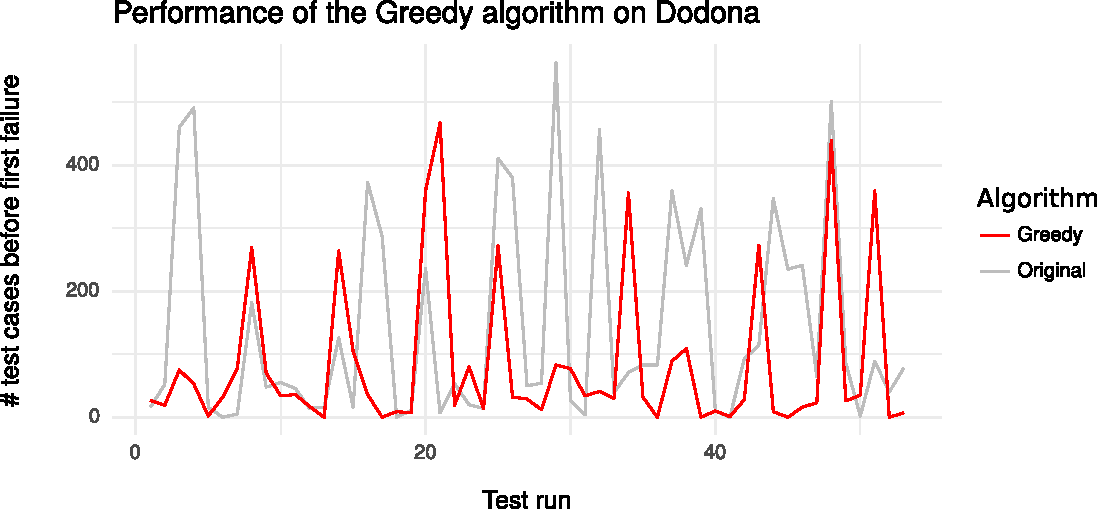
\includegraphics[width=\textwidth]{assets/charts/rq4-dodona-greedy.pdf}
}
\end{figure}
\begin{figure}
\ContinuedFloat
\subfloat[HGS algorithm]{%
	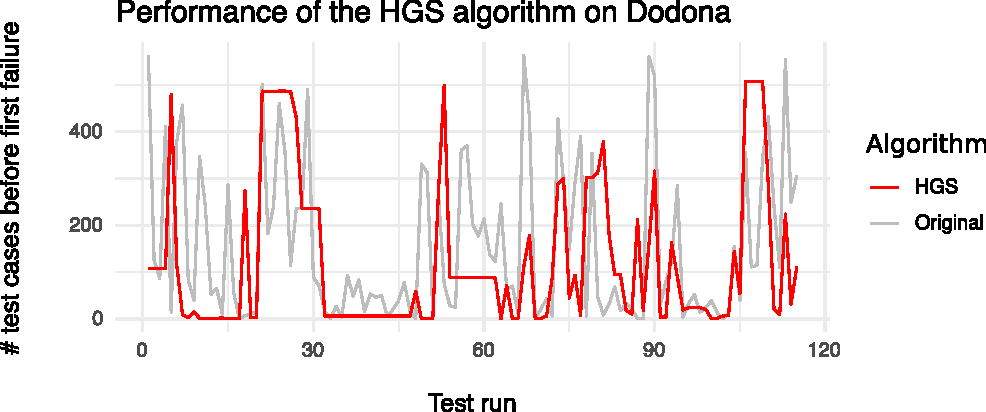
\includegraphics[width=\textwidth]{assets/charts/rq4-dodona-hgs.pdf}
}
\end{figure}
\begin{figure}
\ContinuedFloat
\centering
\subfloat[ROCKET algorithm]{%
	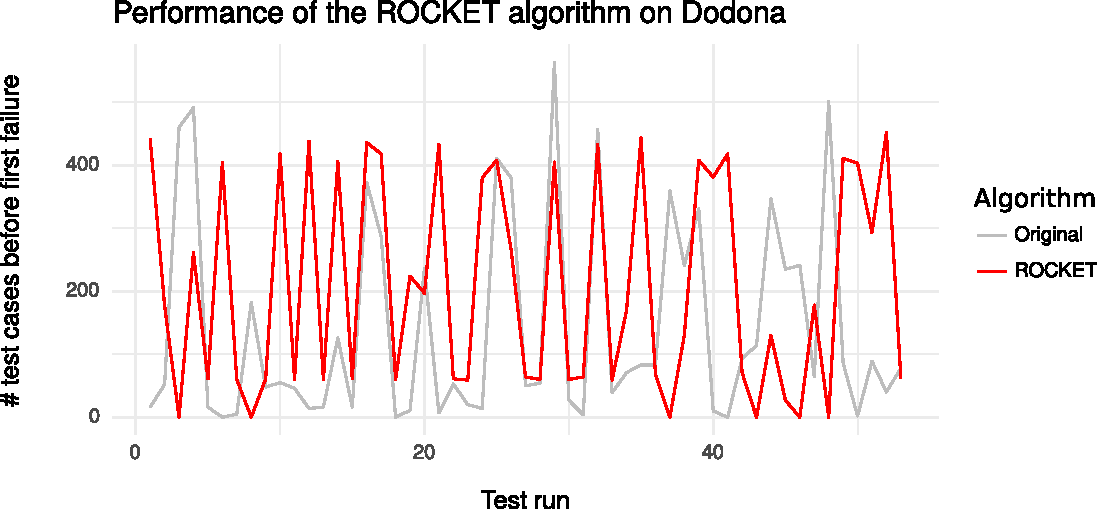
\includegraphics[width=\textwidth]{assets/charts/rq4-dodona-rocket.pdf}
}
\caption{Prediction performance on the Dodona project}
\label{fig:rq4-performance}
\end{figure}

\noindent \autoref{tbl:rq4-first-failure} contains the minimum, mean, median and maximum median amount of test cases until the first failure is observed. This table indicates that, except for the GreedyCoverAffected algorithm\footnote{The AllInOrder algorithm can be considered a deterministic random algorithm and therefore not an actual predictor.}, every predictor is able to perform at least one successful prediction. Furthermore, the maximum amount of executed test cases is lower than the original, for every predictor. The previous paragraph has already observed that the Alpha and HGS algorithm provide the best prediction accuracy for Dodona, this hypothesis is confirmed by the low median and mean values for these algorithms. These values confirm as well that the ROCKET algorithm is not able of providing accurate predictions.

\begin{table}[h]
	\centering
	\begin{tabularx}{\textwidth}{|X||c|c|c|c|}
		\hline
		\textbf{Algorithm} & \textbf{Minimum} & \textbf{Mean} & \textbf{Median} & \textbf{Maximum}\\
		
		\hline
		
		\emph{Original} & $\SI{0}{}$ & $\SI{143}{}$ & $\SI{65}{}$ & $\SI{563}{}$\\
		
		\hline
		
		Alpha & $\SI{0}{}$ & $\SI{7}{}$ & $\SI{6}{}$ & $\SI{44}{}$\\
		
		\hline
		AffectedRandom & $\SI{0}{}$ & $\SI{82}{}$ & $\SI{18}{}$ & $\SI{428}{}$\\
		AllInOrder & $\SI{1}{}$ & $\SI{102}{}$ & $\SI{71}{}$ & $\SI{455}{}$\\
		AllRandom & $\SI{0}{}$ & $\SI{71}{}$ & $\SI{16}{}$ & $\SI{477}{}$\\
		
		\hline
		
		GreedyCoverAffected & $\SI{31}{}$ & $\SI{307}{}$ & $\SI{296}{}$ & $\SI{446}{}$\\
		GreedyCoverAll & $\SI{0}{}$ & $\SI{85}{}$ & $\SI{32}{}$ & $\SI{467}{}$\\
		GreedyTimeAll & $\SI{0}{}$ & $\SI{209}{}$ & $\SI{172}{}$ & $\SI{452}{}$\\
		
		\hline
		
		HGSAffected & $\SI{0}{}$ & $\SI{54}{}$ & $\SI{10}{}$ & $\SI{511}{}$\\
		HGSAll & $\SI{0}{}$ & $\SI{109}{}$ & $\SI{6}{}$ & $\SI{487}{}$\\
		
		\hline
		
		ROCKET & $\SI{0}{}$ & $\SI{208}{}$ & $\SI{170}{}$ & $\SI{452}{}$\\
		
		\hline
	\end{tabularx}
	\caption{Amount of executed test cases until the first failure.}
	\label{tbl:rq4-first-failure}
\end{table}

\noindent Similarly, \autoref{tbl:rq4-first-failure-duration} contains the minimum, mean, maximum and median duration until the first failed test case is observed. This data further confirms the observations made in the previous paragraph and the effectiveness of the GreedyTimeAll predictor. Notice that the ROCKET algorithm performs better time-wise than quantity wise.

\begin{table}[h]
	\centering
	\begin{tabularx}{\textwidth}{|X||c|c|c|c|}
		\hline
		\textbf{Algorithm} & \textbf{Minimum} & \textbf{Mean} & \textbf{Median} & \textbf{Maximum}\\
		
		\hline
		
		\emph{Original} & $\SI{0}{\second}$ & $\SI{154}{\second}$ & $\SI{125}{\second}$ & $\SI{622}{\second}$\\
		
		\hline
		
		Alpha & $\SI{0}{\second}$ & $\SI{5}{\second}$ & $\SI{0}{\second}$ & $\SI{84}{\second}$\\
		
		\hline
		AffectedRandom & $\SI{0}{\second}$ & $\SI{64}{\second}$ & $\SI{10}{\second}$ & $\SI{355}{\second}$\\
		AllInOrder & $\SI{0}{\second}$ & $\SI{177}{\second}$ & $\SI{171}{\second}$ & $\SI{456}{\second}$\\
		AllRandom & $\SI{0}{\second}$ & $\SI{64}{\second}$ & $\SI{11}{\second}$ & $\SI{611}{\second}$\\
		
		\hline
		
		GreedyCoverAffected & $\SI{6}{\second}$ & $\SI{123}{\second}$ & $\SI{109}{\second}$ & $\SI{264}{\second}$\\
		GreedyCoverAll & $\SI{0}{\second}$ & $\SI{60}{\second}$ & $\SI{25}{\second}$ & $\SI{306}{\second}$\\
		GreedyTimeAll & $\SI{0}{\second}$ & $\SI{44}{\second}$ & $\SI{15}{\second}$ & $\SI{178}{\second}$\\
		
		\hline
		
		HGSAffected & $\SI{0}{\second}$ & $\SI{58}{\second}$ & $\SI{6}{\second}$ & $\SI{581}{\second}$\\
		HGSAll & $\SI{0}{\second}$ & $\SI{130}{\second}$ & $\SI{16}{\second}$ & $\SI{578}{\second}$\\
		
		\hline
		
		ROCKET & $\SI{0}{\second}$ & $\SI{47}{\second}$ & $\SI{16}{\second}$ & $\SI{178}{\second}$\\
		
		\hline
	\end{tabularx}
	\caption{Duration until the first failure.}
	\label{tbl:rq4-first-failure-duration}
\end{table}

    duration         Original        AllRandom     
Min.   :118165   Min.   :  0.00   Min.   : 0.000  
1st Qu.:195877   1st Qu.:  0.00   1st Qu.: 0.000  
Median :297371   Median :  2.00   Median : 4.000  
Mean   :303527   Mean   : 67.57   Mean   : 9.257  
3rd Qu.:414956   3rd Qu.:110.00   3rd Qu.:13.500  
Max.   :505996   Max.   :278.00   Max.   :64.000  

AllInOrder     GreedyCoverAll   AffectedRandom  
Min.   : 0.000   Min.   : 0.000   Min.   : 0.000  
1st Qu.: 0.000   1st Qu.: 0.000   1st Qu.: 0.000  
Median : 1.000   Median : 1.000   Median : 2.000  
Mean   : 9.229   Mean   : 8.971   Mean   : 8.886  
3rd Qu.:12.000   3rd Qu.:13.000   3rd Qu.:11.500  
Max.   :37.000   Max.   :44.000   Max.   :45.000  

HGSAffected     GreedyCoverAffected     HGSAll    
Min.   : 0.000   Min.   : 0.00       Min.   : 0.0  
1st Qu.: 0.000   1st Qu.: 0.00       1st Qu.: 0.0  
Median : 3.000   Median : 2.00       Median : 7.0  
Mean   : 8.886   Mean   :15.09       Mean   : 9.6  
3rd Qu.:11.500   3rd Qu.:31.00       3rd Qu.:12.5  
Max.   :64.000   Max.   :43.00       Max.   :43.0  

Alpha            Rocket       GreedyTimeAll   
Min.   : 0.000   Min.   :  0.00   Min.   :  0.00  
1st Qu.: 0.000   1st Qu.:  3.50   1st Qu.:  3.50  
Median : 1.000   Median : 27.00   Median : 27.00  
Mean   : 8.971   Mean   : 42.23   Mean   : 42.23  
3rd Qu.:13.000   3rd Qu.: 49.00   3rd Qu.: 49.00  
Max.   :44.000   Max.   :216.00   Max.   :216.00  

Original\_ms      AllRandom\_ms    AllInOrder\_ms   
Min.   :     0   Min.   :     0   Min.   :     0  
1st Qu.:     0   1st Qu.:     0   1st Qu.:     0  
Median :  9560   Median :   739   Median :   862  
Mean   : 73612   Mean   : 13299   Mean   : 32391  
3rd Qu.:122586   3rd Qu.: 13592   3rd Qu.: 78063  
Max.   :283433   Max.   :184805   Max.   :139345  

GreedyCoverAll\_ms AffectedRandom\_ms HGSAffected\_ms  
Min.   :     0    Min.   :     0    Min.   :     0  
1st Qu.:     0    1st Qu.:     0    1st Qu.:     0  
Median :   620    Median :   317    Median :  1318  
Mean   : 15251    Mean   : 19732    Mean   : 23738  
3rd Qu.:  8620    3rd Qu.:  6460    3rd Qu.: 11786  
Max.   :197463    Max.   :174491    Max.   :211702  

GreedyCoverAffected\_ms   HGSAll\_ms         Alpha\_ms     
Min.   :    0          Min.   :     0   Min.   :     0  
1st Qu.:    0          1st Qu.:     0   1st Qu.:     0  
Median : 4229          Median :  2818   Median :   647  
Mean   :21835          Mean   : 12494   Mean   : 15189  
3rd Qu.:37885          3rd Qu.:  8475   3rd Qu.:  8386  
Max.   :75637          Max.   :157003   Max.   :193618  

Rocket\_ms      GreedyTimeAll\_ms      idx      
Min.   :     0   Min.   :    0    Min.   : 1.0  
1st Qu.:     0   1st Qu.:    0    1st Qu.: 9.5  
Median :   254   Median :  257    Median :18.0  
Mean   :  6844   Mean   : 6852    Mean   :18.0  
3rd Qu.:  1760   3rd Qu.: 1754    3rd Qu.:26.5  
Max.   :100011   Max.   :99765    Max.   :35.0  
